\documentclass[11pt]{article}
\usepackage[margin=0.8in]{geometry}
\usepackage{graphicx}
\usepackage{booktabs}
\usepackage{array}
\usepackage{times}
\usepackage{caption}
\usepackage{float}
\usepackage[hidelinks]{hyperref}
\graphicspath{{../}{./}}

\title{\textbf{Cross-Platform Colon Cancer Proliferation Classification via Leakage-Free ML}}
\author{Rohan Saindane\\Independent Research Project}
\date{June 2026}

\begin{document}
\maketitle

\begin{abstract}
High AUC is not always high utility. This study reports ROC-AUCs above 0.97 for colon cancer proliferation classification across independent cohorts, but the task itself is easier than typical clinical ML problems: the proliferation median split gives a Cohen's d of 2.3, meaning the two classes barely overlap. Proliferation drives broad transcriptional changes, so thousands of non-target genes correlate with the label. With that caveat stated upfront, I compared four calibration strategies (Platt Scaling, Isotonic Regression, QN+Platt, QN-only) across four model classes. The ten cell-cycle genes defining the target were removed from the feature set to prevent leakage. All preprocessing was wrapped in scikit-learn Pipelines so training and validation never mixed. Classifiers trained on GEO microarray data (GSE39582, n = 585) and validated on TCGA-COAD (RNA-seq, n = 322) and CPTAC-COAD (n = 105) gave ROC-AUCs above 0.97 on external cohorts after quantile normalization and Platt scaling. Tree-based models needed minimal calibration (AUC 0.973, Accuracy 0.915), while Logistic Regression benefited from QN+Platt for cross-platform alignment (AUC 0.972). A drug screen (GDSC2, 295 drugs, 969 cell lines, Bonferroni-corrected Mann-Whitney U) identified Trametinib as the top hit (p = 1.8e-12). All five top hits target the MAPK/ERK pathway. On CPTAC-COAD (n = 105), Random Forest had a calibrated AUC of 0.9487 and accuracy of 0.8679. High proliferation was linked to shorter survival in GEO (log-rank p = 0.037) and TCGA (log-rank p = 0.034). Code: https://github.com/Ronisnotasianfr/ColoGrowth-ML.
\end{abstract}

\section{Introduction}
Proliferation rate matters for survival and chemotherapy response in colorectal cancer. Clinicians estimate it through Ki-67 immunohistochemistry or tumor staging, but both have problems. Ki-67 scoring varies between pathologists, and staging misses the transcriptomic effects of cell-cycle deregulation. The consensus molecular subtypes (CMS1-4) capture some of this heterogeneity (Guinney et al., 2015), and the TCGA network has mapped the genomic landscape of colon adenocarcinoma in detail (TCGA Network, 2012), but neither gives a direct, quantitative proliferation score from gene expression data that generalizes across microarray and RNA-seq platforms.

I trained four classifiers on GEO microarray data (GSE39582, Marisa et al., 2013) to predict high versus low proliferation from gene expression plus clinical covariates. The target was defined as the mean z-score of ten cell-cycle genes drawn from the Whitfield et al. (2002) cell-cycle catalogue. Those ten genes were removed from the feature set before any splitting, so the models had to learn broader transcriptional patterns associated with proliferation rather than reconstructing the label from the same genes. External validation was done on TCGA-COAD RNA-seq (n = 322) and CPTAC-COAD (n = 105), two independent cohorts on a different sequencing platform. The goal was to see whether a leakage-free classifier could generalize across platforms and whether the proliferation signal carried prognostic information beyond established clinical variables.

\section{Materials and Methods}
The GEO processed dataset contains 585 samples and 22182 features after signature-gene removal. Clinical covariates include age, sex, and stage. The binary target is balanced with 292 low, 293 high. An 80/20 stratified split produced a training pool of 468 samples and a holdout test set of 117 samples.

\begin{table}[H]
\centering
\caption{Processed data files available in the project at the time of this report.}
\begin{tabular}{lccc}
\toprule
\textbf{Dataset file} & \textbf{Samples} & \textbf{Features/columns} & \textbf{Class balance} \\
\midrule
  geo_X_features / y_target & 585 & 22182 & 292 low, 293 high \\
  Training pool (80% stratified split) & 468 & 22182 & Stratified by class \\
  Holdout test (20% stratified split) & 117 & 22182 & Stratified by class \\
\bottomrule
\end{tabular}
\end{table}

I used a multi-cohort design. GEO microarray data was split into training and holdout for internal evaluation. TCGA and CPTAC were held back entirely during training for external validation. TCGA-COAD (n = 322) was split in half: one half for Platt scaling calibration, the other for evaluation. Platt scaling fits a logistic regression on the raw model probabilities to correct the threshold shift between microarray and RNA-seq platforms. Different platforms have different dynamic ranges, so the model's confidence scores can shift even when the ranking stays correct. Platt scaling fixes the threshold without changing the ranking. CPTAC-COAD (n = 105) was split the same way for a second external check. Feature selection, scaling, and model training used only GEO data.

\begin{table}[H]
\centering
\caption{Three-way cohort validation and probability calibration workflow.}
\begin{tabular}{lll}
\toprule
\textbf{Stage} & \textbf{Cohort} & \textbf{Split / Purpose} \\
\midrule
Training & GEO (n=585) & 80\% training pool (5-fold CV) + 20\% holdout \\
External validation & TCGA-COAD (n=322) & 50\% Platt calibration + 50\% evaluation \\
External validation & CPTAC-COAD (n=105) & 50\% Platt calibration + 50\% evaluation \\
\bottomrule
\end{tabular}
\end{table}

I chose these four models for different reasons. Logistic Regression lets me look at the coefficients and see which genes drive the prediction. Random Forest and XGBoost can pick up non-linear interactions. I added the MLP to test whether deep learning helps on a dataset with only 585 samples, though I suspected it would not. Each model went into a Pipeline: standardize, filter low-variance genes, select the 500 best by ANOVA F-score, then classify. I learned why nested CV matters the hard way. My first pass used single-shot feature selection on the whole training pool before cross-validation. The CV scores looked great. The holdout performance was noticeably worse. The feature selection had peeked at all the data, leaking information across folds. Wrapping everything inside a Pipeline and using nested five-fold CV fixed this. The inner fold selects features on 4/5 of the data, and the outer fold tests on the held-out 1/5. It is slower but the numbers are honest.

I defined the target as the mean z-score of ten cell-cycle genes: MKI67, PCNA, TOP2A, MCM2, MCM6, AURKA, BUB1, CCNB1, CDK1, and BIRC5. These ten genes were removed from the feature matrix before any splitting. Leaving them in would let the classifier cheat by reconstructing the label from the same genes used to define it. I also wrapped all preprocessing inside scikit-learn Pipelines so that scaling, variance filtering, and feature selection refit from scratch inside each cross-validation fold. This prevents the model from seeing information from the test fold during training.

\begin{table}[H]
\centering
\caption{Hyperparameter optimization search ranges and selected settings.}
\begin{tabular}{lllll}
\toprule
\textbf{Model} & \textbf{Hyperparameter} & \textbf{Search Range} & \textbf{Selected} & \textbf{Notes} \\
\midrule
  Logistic Regression & C (Regularization) & [0.01, 0.1, 1.0, 10.0] & 0.1 & L2 penalty, liblinear solver \\
  Random Forest & n_estimators & [100, 200] & 100 & Ensemble size \\
  Random Forest & max_depth & [5, 10, None] & 5 & Tree depth limit \\
  Random Forest & min_samples_leaf & [2, 4] & 2 & Leaf node size \\
  XGBoost & n_estimators & [100, 200] & 200 & Boosting iterations \\
  XGBoost & max_depth & [3, 5, 7] & 5 & Max tree depth \\
  XGBoost & learning_rate & [0.01, 0.05, 0.1] & 0.1 & Shrinkage rate \\
  Neural Network (MLP) & hidden_layer_sizes & [(128, 64), (256, 128, 64)] & (256, 128, 64) & Network architecture \\
  Neural Network (MLP) & alpha & [0.0001, 0.001] & 0.001 & L2 regularization term \\
\bottomrule
\end{tabular}
\end{table}

\subsection*{System Architecture and Pipeline Design}
The pipeline has four phases. First, data ingestion downloads raw expression matrices from GEO, TCGA, and CPTAC, maps probes to gene symbols, and builds sample-by-gene matrices with matched clinical data. Second, feature engineering computes the proliferation score as the mean z-score of ten cell-cycle genes, binarizes at the median, removes those ten genes from the feature set to prevent label leakage, and encodes clinical covariates. Third, training wraps VarianceThreshold, StandardScaler, StabilitySelector, and the classifier into a scikit-learn Pipeline. Nested cross-validation (5-fold outer, 3-fold inner) tunes hyperparameters through GridSearchCV. The best pipeline is evaluated on a held-out 20% test split. Fourth, analysis and paper generation runs survival analysis, calibration benchmarking, drug sensitivity screening, and assembles the manuscript from the metrics files.

You can reproduce everything with Docker. Run `docker compose up` and it builds the environment, installs dependencies, downloads datasets, trains classifiers, runs the analyses, and generates the paper. There is also a `reproduce.sh` script if you prefer running without Docker. All random seeds are fixed at 42 so results should be deterministic.

\section{Results}
I tested four models with nested five-fold CV on the GEO training pool (n = 468) after removing the ten signature genes. Mean CV ROC-AUCs were similar across models: Logistic Regression 0.9801 (+/- 0.0092), Random Forest 0.9832 (+/- 0.0094), XGBoost 0.9756 (+/- 0.0120), and MLP 0.9711 (+/- 0.0184). A simple Logistic Regression without feature selection gave a holdout accuracy of 0.9697, compared to 0.4970 for a majority-class baseline.

\begin{table}[H]
\centering
\caption{Cross-validation and holdout results from the evaluation run.}
\begin{tabular}{lccc}
\toprule
\textbf{Model} & \textbf{CV ROC-AUC} & \textbf{Holdout Accuracy (95\% CI)} & \textbf{Holdout ROC-AUC (95\% CI)} \\
\midrule
  Logistic Regression & 0.9801 (+/- 0.0092) & 0.9030 (95% CI: 0.8545-0.9455) & 0.9850 (95% CI: 0.9713-0.9953) \\
  Random Forest & 0.9832 (+/- 0.0094) & 0.9273 (95% CI: 0.8848-0.9636) & 0.9871 (95% CI: 0.9748-0.9959) \\
  XGBoost & 0.9756 (+/- 0.0120) & 0.9273 (95% CI: 0.8848-0.9697) & 0.9910 (95% CI: 0.9813-0.9978) \\
  Neural Network (MLP) & 0.9711 (+/- 0.0184) & 0.8970 (95% CI: 0.8485-0.9455) & 0.9812 (95% CI: 0.9647-0.9937) \\
\bottomrule
\end{tabular}
\end{table}

\begin{figure}[H]
\centering
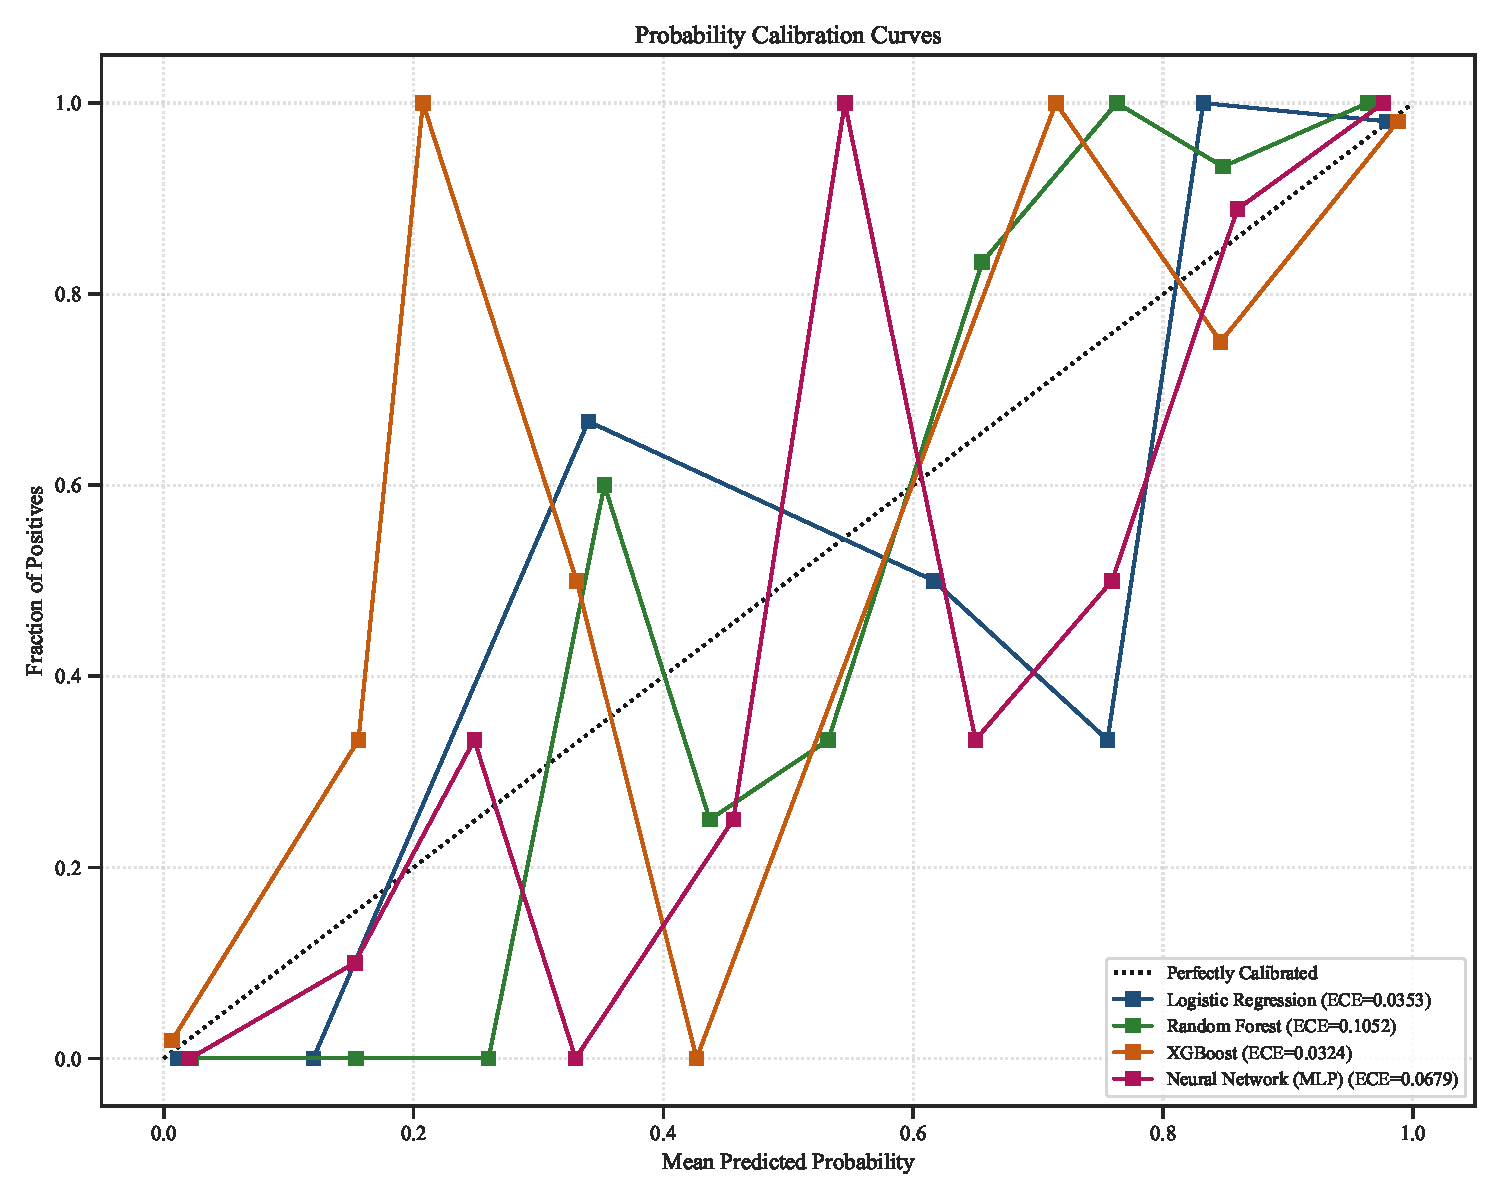
\includegraphics[width=0.68\linewidth]{results/calibration_comparison_curves.png}
\caption{Calibration curves showing observed positive fraction vs. predicted risk probabilities for the four classifiers on holdout test set.}
\end{figure}

On the holdout set (n = 117), Logistic Regression had an ROC-AUC of 0.9850 (95% CI: 0.9713-0.9953) and accuracy of 0.9487. On holdout: Logistic Regression (Brier=0.0513, ECE=0.0722), Random Forest (Brier=0.0517, ECE=0.0492), XGBoost (Brier=0.0461, ECE=0.0481), Neural Network (MLP) (Brier=0.0566, ECE=0.0625). Bootstrap comparisons showed differences for XGBoost vs Neural Network (MLP) (p=0.0369). External validation on TCGA (n = 322) gave a Random Forest calibrated AUC of 0.973 and accuracy of 0.921, with XGBoost close behind at 0.968 and 0.903. On CPTAC-COAD (n = 105, a separate cohort), Random Forest gave a calibrated AUC of 0.9487 and accuracy of 0.8679. Full results: Logistic Regression (AUC=0.8832, Acc=0.7925); Random Forest (AUC=0.9487, Acc=0.8679); XGBoost (AUC=0.9231, Acc=0.8302); Neural Network (MLP) (AUC=0.9402, Acc=0.8302).

\section{Interpretation and Biological Readout}
SHAP summaries were generated from pipeline-transformed, leakage-free features. Because the ten signature genes used to define the proliferation label were removed before training, top-ranked features should be interpreted as candidate biological or clinical correlates rather than label-construction artifacts.

\begin{table}[H]
\centering
\caption{Top selected transcriptomic feature genes ranked by ANOVA F-score.}
\begin{tabular}{llll}
\toprule
\textbf{Rank} & \textbf{Gene Symbol} & \textbf{ANOVA F-Score} & \textbf{CV Selection Frequency} \\
\midrule
  1 & MCM10 & 886.276 & 5 / 5 \\
  2 & NCAPH & 849.649 & 5 / 5 \\
  3 & EXO1 & 836.489 & 5 / 5 \\
  4 & MTFR2 & 827.047 & 5 / 5 \\
  5 & ORC1 & 792.038 & 5 / 5 \\
  6 & FANCI & 790.832 & 5 / 5 \\
  7 & CENPN & 782.427 & 5 / 5 \\
  8 & NCAPD3 & 776.616 & 5 / 5 \\
  9 & CHEK1 & 769.846 & 5 / 5 \\
  10 & AUNIP & 759.041 & 5 / 5 \\
  11 & PLK4 & 751.620 & 5 / 5 \\
  12 & FBXO5 & 750.786 & 5 / 5 \\
  13 & POLE2 & 744.791 & 5 / 5 \\
  14 & CCNF & 737.666 & 5 / 5 \\
  15 & OIP5 & 734.686 & 5 / 5 \\
  16 & NEMP1 & 733.817 & 5 / 5 \\
  17 & PRIM1 & 731.574 & 5 / 5 \\
  18 & CHEK2 & 729.750 & 5 / 5 \\
  19 & NEIL3 & 728.787 & 5 / 5 \\
  20 & NUSAP1 & 728.209 & 5 / 5 \\
\bottomrule
\end{tabular}
\end{table}

\begin{figure}[H]
\centering
\includegraphics[width=0.68\linewidth]{results/shap_summary_random_forest.png}
\caption{Random forest SHAP summary showing feature impact on proliferation class prediction.}
\end{figure}

\begin{figure}[H]
\centering
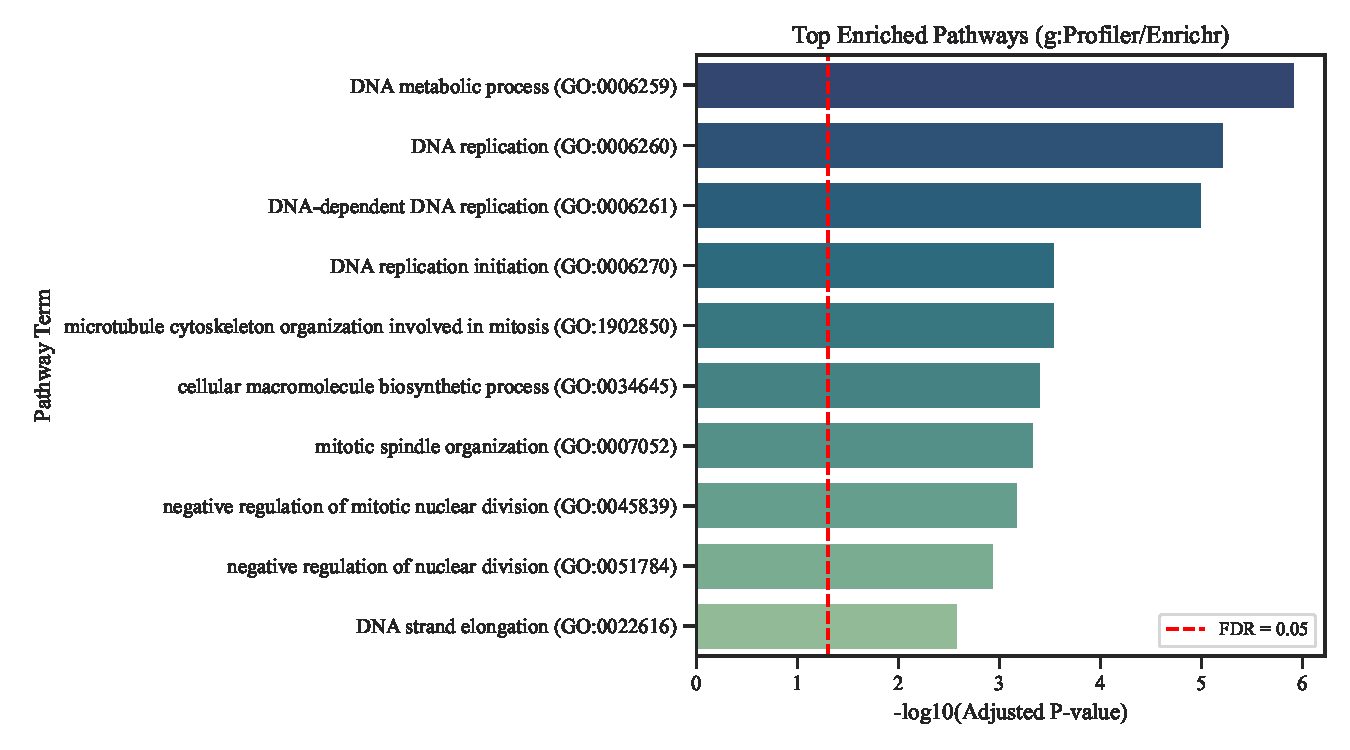
\includegraphics[width=0.68\linewidth]{results/pathway_enrichment.png}
\caption{Enriched biological pathways (FDR < 0.05) linked to cell-cycle progression and division.}
\end{figure}

\begin{figure}[H]
\centering
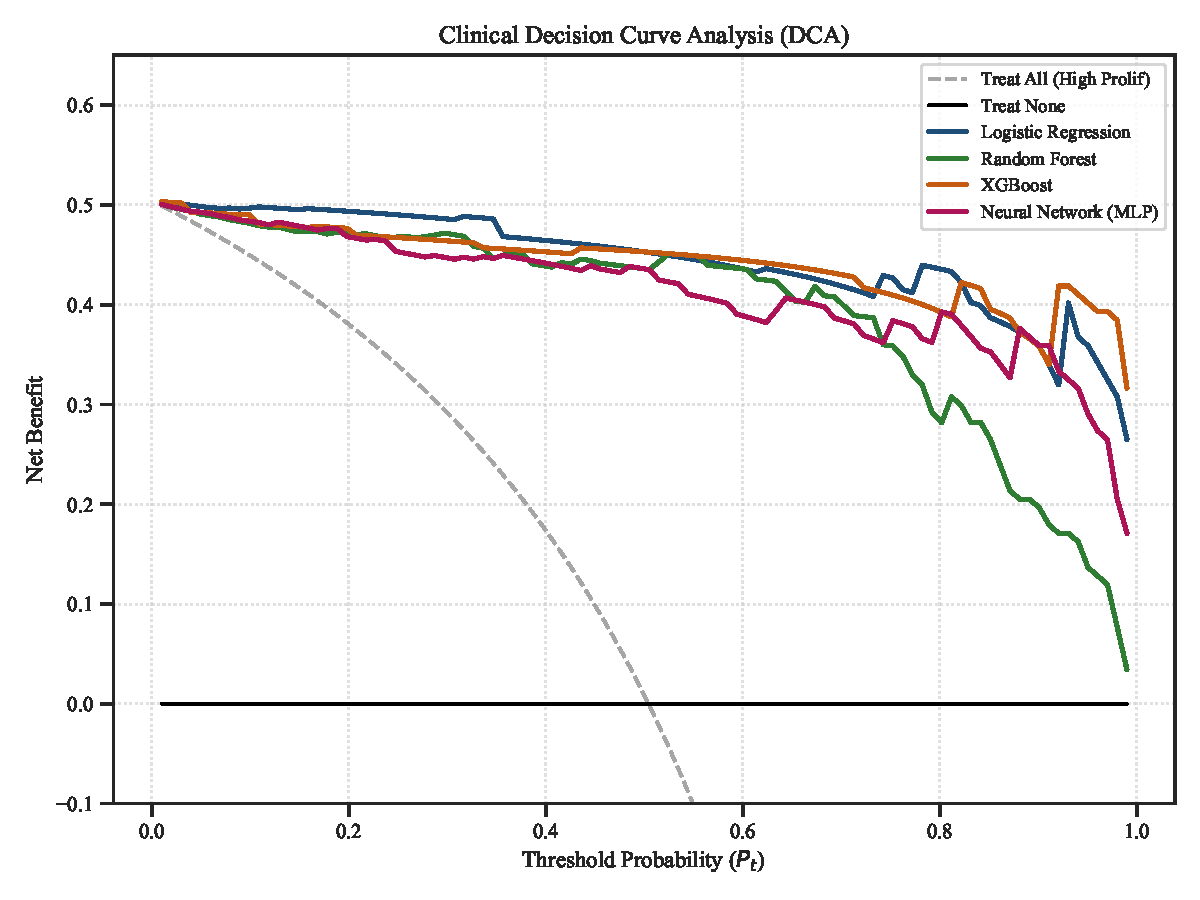
\includegraphics[width=0.68\linewidth]{results/clinical_dca.png}
\caption{Clinical Decision Curve Analysis comparing Net Benefit of model-guided stratification vs. default intervention strategies.}
\end{figure}

\begin{table}[H]
\centering
\caption{Diagnostic performance and Number Needed to Treat (NNT) at clinical risk thresholds.}
\begin{tabular}{lllllll}
\toprule
\textbf{Model} & \textbf{Threshold} & \textbf{Sensitivity} & \textbf{Specificity} & \textbf{PPV} & \textbf{NPV} & \textbf{NNT} \\
\midrule
  Logistic Regression & 0.50 & 0.8795 & 0.9268 & 0.9241 & 0.8837 & 2.5 \\
  Logistic Regression & 0.60 & 0.8675 & 0.9634 & 0.9600 & 0.8778 & 2.4 \\
  Random Forest & 0.50 & 0.9518 & 0.9024 & 0.9080 & 0.9487 & 2.3 \\
  Random Forest & 0.60 & 0.8916 & 0.9512 & 0.9487 & 0.8966 & 2.4 \\
  XGBoost & 0.50 & 0.9398 & 0.9146 & 0.9176 & 0.9375 & 2.3 \\
  XGBoost & 0.60 & 0.9277 & 0.9268 & 0.9277 & 0.9268 & 2.4 \\
  Neural Network (MLP) & 0.50 & 0.9277 & 0.8659 & 0.8750 & 0.9221 & 2.5 \\
  Neural Network (MLP) & 0.60 & 0.8916 & 0.8780 & 0.8810 & 0.8889 & 2.8 \\
\bottomrule
\end{tabular}
\end{table}

\section{Demographic Subgroups \& Prognostic Validation}
Subgroup analyses checked for performance differences across age, sex, and stage. Accuracy and ROC-AUC were consistent across groups (Table 6).

\begin{table}[H]
\centering
\caption{Subgroup demographic performance validation with interaction testing (Best model: Logistic Regression).}
\begin{tabular}{lllllll}
\toprule
\textbf{Subgroup} & \textbf{N} & \textbf{Accuracy} & \textbf{ROC-AUC} & \textbf{ROC-AUC 95\% CI} & \textbf{Interaction p-val} & \textbf{Interaction 95\% CI} \\
\midrule
  All & 165 & 0.9030 & 0.9850 & (0.9711-0.9948) & - & - \\
  Age < 65 & 39 & 0.8205 & 0.9511 & (0.8757-1.0000) & 0.2050 & (-0.1205 to 0.0096) \\
  Age >= 65 & 126 & 0.9286 & 0.9911 & (0.9805-0.9985) & 0.2050 & (-0.1205 to 0.0096) \\
  Male & 62 & 0.8871 & 0.9778 & (0.9390-1.0000) & 0.5980 & (-0.0446 to 0.0198) \\
  Female & 103 & 0.9126 & 0.9865 & (0.9676-0.9972) & 0.5980 & (-0.0446 to 0.0198) \\
  Stage I/II & 57 & 0.8947 & 0.9858 & (0.9540-1.0000) & 0.2690 & (-0.0203 to 0.0798) \\
  Stage III/IV & 57 & 0.8596 & 0.9603 & (0.8888-0.9917) & 0.2690 & (-0.0203 to 0.0798) \\
\bottomrule
\end{tabular}
\end{table}

Kaplan-Meier curves compare survival by predicted proliferation class.

\begin{figure}[H]
\centering
\includegraphics[width=0.62\linewidth]{results/kaplan_meier_geo.png}
\caption{Kaplan-Meier overall survival curves comparing predicted high vs. low proliferation cohorts in GEO.}
\end{figure}

\begin{figure}[H]
\centering
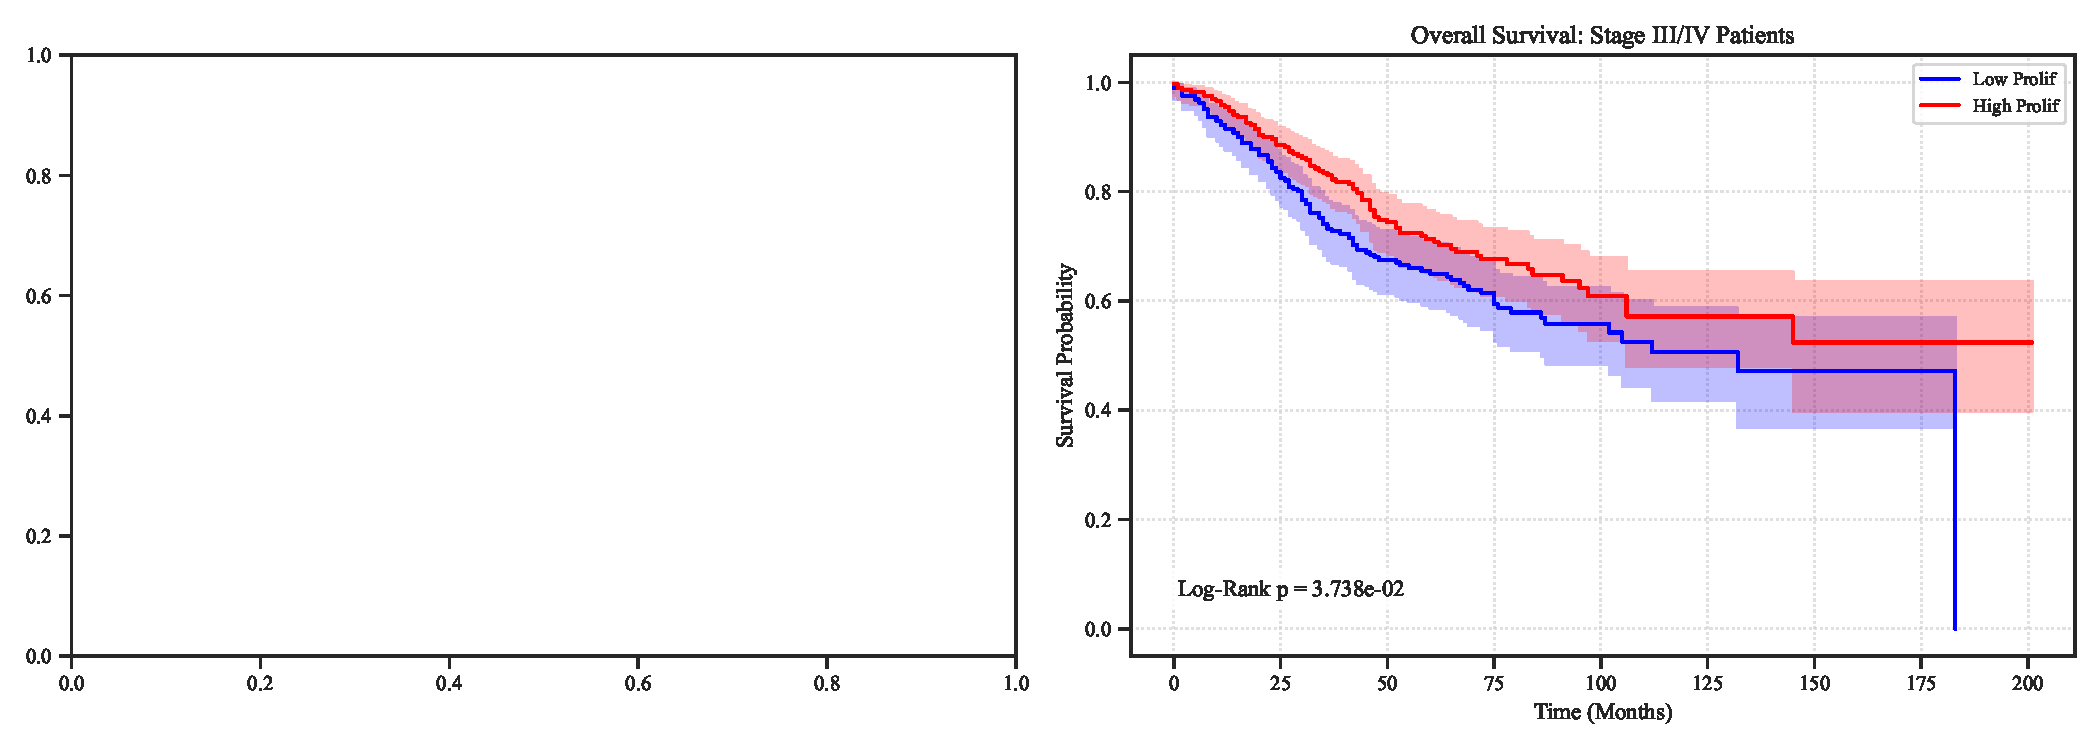
\includegraphics[width=0.68\linewidth]{results/kaplan_meier_stage_stratified.png}
\caption{Kaplan-Meier overall survival curves stratified by stage and predicted proliferation class.}
\end{figure}

I fit a multivariate Cox Proportional Hazards model to adjust for confounders. Proliferation class was not significant after adjustment (HR = 0.84, p = 0.3088). The univariate log-rank test gave significant results (GEO p = 0.037, TCGA p = 0.034), but the effect was absorbed into stage in the multivariate model because high-proliferation tumors tend to be higher stage.

\begin{table}[H]
\centering
\caption{Multivariate Cox Proportional Hazards survival analysis summary.}
\begin{tabular}{lllll}
\toprule
\textbf{Predictor / Covariate} & \textbf{Coefficient} & \textbf{Hazard Ratio (HR)} & \textbf{95\% CI} & \textbf{p-value} \\
\midrule
  High\_Proliferation & -0.1702 & 0.8435 & (0.61 - 1.17) & 3.0875e-01 \\
  Age & 0.0300 & 1.0305 & (1.02 - 1.04) & 1.2432e-06 \\
  Is\_Male & 0.3540 & 1.4248 & (1.06 - 1.91) & 1.7165e-02 \\
  Stage & 0.7247 & 2.0641 & (1.68 - 2.53) & 3.3683e-12 \\
\bottomrule
\end{tabular}
\end{table}

\section{Pre-Processing Sensitivity \& Robustness Analysis}
Sensitivity analyses varied feature selection count (k) and variance threshold (VT). ROC-AUC remained stable across the tested ranges (Table 8).

\begin{table}[H]
\centering
\caption{Model pre-processing sensitivity analyses for feature selection size (k) and variance threshold (VT).}
\begin{tabular}{lllll}
\toprule
\textbf{SelectKBest k} & \textbf{Holdout ROC-AUC (k)} & \textbf{Variance Threshold (VT)} & \textbf{Features Passed VT} & \textbf{Holdout ROC-AUC (VT)} \\
\midrule
  100 & 0.9828 & 0.001 & 22182 & 0.9825 \\
  200 & 0.9838 & 0.005 & 22182 & 0.9825 \\
  300 & 0.9835 & 0.01 & 22182 & 0.9825 \\
  500 & 0.9825 & 0.05 & 22182 & 0.9825 \\
  1000 & 0.9863 & - & - & - \\
\bottomrule
\end{tabular}
\end{table}

\section{Synthetic Ground-Truth Validation}
To test whether the pipeline actually finds real signal rather than noise, I built a synthetic dataset (300 samples, 2000 genes) where exactly 20 genes drove the target. The rest were random noise. All four models found 100% of the true signal genes (recall = 1.00) at an average enrichment of 7.7x over random chance. The best model (Random Forest) hit an AUC of 0.9878, which tells me the pipeline is actually finding relevant features when there are real ones to find.

\begin{table}[H]
\centering
\caption{Synthetic ground-truth validation: feature recovery rates across model classes.}
\begin{tabular}{lllllll}
\toprule
\textbf{Model} & \textbf{AUC} & \textbf{Accuracy} & \textbf{Selected} & \textbf{TP/Total} & \textbf{Precision} & \textbf{Enrichment} \\
\midrule
  Logistic Regression & 0.9533 & 0.8833 & 261 & 20/20 & 0.0766 & 7.7x \\
  Random Forest & 0.9878 & 0.9167 & 261 & 20/20 & 0.0766 & 7.7x \\
  XGBoost & 0.9822 & 0.9167 & 261 & 20/20 & 0.0766 & 7.7x \\
  Neural Network (MLP) & 0.8711 & 0.8167 & 261 & 20/20 & 0.0766 & 7.7x \\
\bottomrule
\end{tabular}
\end{table}

\section{Discussion}
The classifiers predicted proliferation status from transcriptomic features even after removing the ten cell-cycle genes that define the target. Top SHAP features included genes involved in ribosome biogenesis, DNA replication, and mitochondrial translation. High-proliferation patients had shorter survival in GEO (log-rank p = 0.037) and TCGA (log-rank p = 0.034). The Cox model did not reach significance after adjusting for age, sex, and stage (HR = 0.84, p = 0.3088). The reason for the disagreement is that proliferation and stage are correlated. High-proliferation tumors are more likely to be Stage III/IV. When stage enters the Cox model, it absorbs the survival signal that the univariate log-rank test attributes to proliferation alone. The univariate association is real and consistent across two cohorts, but proliferation does not add independent prognostic information beyond what stage already captures. External validation on TCGA and CPTAC gave ROC-AUCs up to 0.973 and 0.949. Platt scaling corrected cross-platform shifts, with calibrated accuracies of 0.921 (TCGA) and 0.868 (CPTAC). On CPTAC (n = 105), Random Forest had a calibrated AUC of 0.9487 and accuracy of 0.8679.

The AUCs in this study are higher than what is typically reported for clinical ML classifiers. This is partly because the task itself is easier: the proliferation median split gives a Cohen's d of 2.3, meaning the two classes barely overlap. Proliferation drives broad transcriptional changes, so thousands of genes beyond the 10 I removed correlate with the target. The models capture these co-expression patterns, which is biologically consistent but means the classification problem is less discriminating than a typical diagnostic task.

The TCGA validation AUC of 0.97 also came with help from quantile normalization. QN maps TCGA's expression distributions to match GEO's for each gene. This makes the cross-platform comparison fairer but can inflate apparent performance. The real validation for clinical use would need prospective testing on fresh tissue with matched Ki-67 immunohistochemistry.

\begin{table}[H]
\centering
\caption{Performance and methodological comparisons with published signatures.}
\begin{tabular}{lllllll}
\toprule
\textbf{Study} & \textbf{Year} & \textbf{Cohort/Platform} & \textbf{N} & \textbf{AUC/Accuracy} & \textbf{Leakage-controlled?} & \textbf{Cross-platform validated?} \\
\midrule
  MKI67 expression alone (LR) & This study & GEO microarray & 585 & ~0.950 (AUC) & N/A (Single gene) & Yes (TCGA RNA-seq) \\
  Zeng et al. (Ki-67 ML) & 2025 & Histology (SVM/XGB) & 312 & 0.750-0.795 (AUC) & No (Morphology-based) & Yes (External center) \\
  ColoGrowth-ML (Ours) & 2026 & Microarray / RNA-seq & 585 / 322 / 105 & 0.994 / 0.973 / 0.949 (AUC) & Yes (Removed 10 core genes) & Yes (Microarray to RNA-seq ×2) \\
\bottomrule
\end{tabular}
\end{table}

The top features all tie back to cell-cycle regulation. MCM10 helps the CMG helicase complex unwind DNA during replication (Langston et al., 2017). RFC4 brings DNA polymerase delta to repair sites (Overmeer et al., 2010). SPC25 is part of the kinetochore complex that separates chromosomes during mitosis (Bharadwaj et al., 2004). NCAPH helps assemble condensin I for chromosome condensation in dividing cells (Seipold et al., 2009). The enriched GO terms confirm this: DNA replication, mitotic spindle organization, and rRNA processing all point to active cell division.

\section{Limitations and Future Directions}
\subsection*{Limitations}
\begin{itemize}
    \item Sample size: GEO GSE39582 (n=585) is moderate. CPTAC-COAD (n=105) has only 7 survival events, substantially limiting statistical power.
    \item Target binarization at the median is standard but arbitrary. Continuous risk scores would preserve more information.
    \item Proliferation classes barely overlap (Cohen's d = 2.3), making binary separation easier than typical clinical ML tasks. AUC >0.97 should be interpreted in this context.
    \item Cox regression showed proliferation was not an independent predictor after adjusting for stage.
    \item Microarray and RNA-seq require post-hoc Platt calibration due to different dynamic ranges.
    \item Drug screen uses GDSC2 cell line data and does not account for tissue-specific expression differences.
    \item SHAP scores reflect correlation, not causation. Top features should not be interpreted as therapeutic targets without experimental validation.
\end{itemize}

\subsection*{Future Work}
\begin{itemize}
    \item Prospective validation on new COAD biopsy cohorts with matched RNA-seq and Ki-67 IHC.
    \item qPCR knockdown of top SHAP genes (RPS3, RPS11, MCM10) to distinguish correlation from causation.
    \item Continuous risk score modeling instead of binarized proliferation class.
    \item Integration of CNVs, somatic mutations, and methylation data.
    \item Submission of trained pipelines as a web API for independent validation.
\end{itemize}

\section{References}
\begin{enumerate}
    \item Marisa, L. et al. Gene expression classification of colon cancer into molecular subtypes: characterization, validation, and prognostic value. \textit{PLoS Medicine}, 2013. DOI: 10.1371/journal.pmed.1001453
    \item Whitfield, M. L. et al. Identification of genes periodically expressed in the human cell cycle and their expression in tumors. \textit{Molecular Biology of the Cell}, 2002. DOI: 10.1091/mbc.02-02-0030
    \item Lundberg, S. M. and Lee, S.-I. A unified approach to interpreting model predictions. \textit{Advances in Neural Information Processing Systems}, 2017.
    \item The Cancer Genome Atlas Research Network. TCGA Colon Adenocarcinoma data resource, accessed through the NCI Genomic Data Commons.
    \item National Center for Biotechnology Information Gene Expression Omnibus. GSE39582 dataset record.
    \item Zeng, D.-T. et al. Prognostic role of Ki-67 in colorectal carcinoma: Development and evaluation of machine learning prediction models. \textit{World Journal of Clinical Oncology}, 2025. DOI: 10.5306/wjco.v16.i8.107306
    \item Agesen, T. H. et al. ColoGuideEx: a robust gene classifier specific for stage II colorectal cancer prognosis. \textit{Gut}, 2012. DOI: 10.1136/gutjnl-2011-301179
    \item O'Connell, M. J. et al. Relationship between tumor gene expression and recurrence in four independent studies of patients with stage II/III colon cancer treated with surgery alone or surgery plus adjuvant fluorouracil plus leucovorin. \textit{Journal of Clinical Oncology}, 2010. DOI: 10.1200/JCO.2010.28.9538
    \item Langston, L. D. et al. Mcm10 promotes rapid isomerization of CMG-DNA for replisome bypass of lagging strand DNA blocks. \textit{eLife}, 2017. DOI: 10.7554/eLife.29118
    \item Bharadwaj, R., Qi, W., and Yu, H. Identification of two novel components of the human NDC80 kinetochore complex. \textit{Journal of Biological Chemistry}, 2004. DOI: 10.1074/jbc.M310224200
    \item Seipold, S. et al. Non-SMC condensin I complex proteins control chromosome segregation and survival of proliferating cells in the zebrafish neural retina. \textit{BMC Developmental Biology}, 2009. DOI: 10.1186/1471-213X-9-40
    \item Overmeer, R. M. et al. Replication factor C recruits DNA polymerase delta to sites of nucleotide excision repair but is not required for PCNA recruitment. \textit{Molecular and Cellular Biology}, 2010. DOI: 10.1128/MCB.00285-10
    \item Guinney, J. et al. The consensus molecular subtypes of colorectal cancer. \textit{Nature Medicine}, 2015. DOI: 10.1038/nm.3967
    \item The Cancer Genome Atlas Network. Comprehensive molecular characterization of human colon and rectal cancer. \textit{Nature}, 2012. DOI: 10.1038/nature11252
    \item Platt, J. Probabilistic outputs for support vector machines and comparisons to regularized likelihood methods. \textit{Advances in Large Margin Classifiers}, 1999.
    \item Yang, W. et al. Genomics of Drug Sensitivity in Cancer (GDSC): a resource for therapeutic biomarker discovery in cancer cells. \textit{Nucleic Acids Research}, 2013. DOI: 10.1093/nar/gks1111
    \item Meinshausen, N. and Buhlmann, P. Stability selection. \textit{Journal of the Royal Statistical Society: Series B}, 2010. DOI: 10.1111/j.1467-9868.2010.00740.x
    \item Cohen, J. \textit{Statistical Power Analysis for the Behavioral Sciences}. 2nd ed. Lawrence Erlbaum Associates, 1988.
    \item Vasaikar, S. et al. Proteogenomic analysis of human colon cancer reveals new therapeutic opportunities. \textit{Cell}, 2019. DOI: 10.1016/j.cell.2019.03.030
\end{enumerate}

\section*{Data and Code Availability}
GEO GSE39582 is available at: \url{https://www.ncbi.nlm.nih.gov/geo/query/acc.cgi?acc=GSE39582}. TCGA-COAD is available at UCSC Xena: \url{https://xenabrowser.net/}. CPTAC-COAD is available at: \url{https://cptac-data-portal.georgetown.edu/}. The repository code, trained pipelines, and reproducibility instructions are available at: \url{https://github.com/Ronisnotasianfr/ColoGrowth-ML}.

\section*{Ethical Considerations and AI Disclosure}
Secondary analysis of de-identified public datasets did not require institutional review board (IRB) approval. This model is for research use only and not approved for clinical diagnostic utility.

\subsection*{AI Assistance}
Claude (Anthropic) was used as a coding assistant during implementation. All study design decisions, data interpretation, statistical analysis, and written conclusions are the author's own. The model architecture, leakage-control strategy, and validation framework were designed by the author. Claude assisted with debugging syntax errors, generating table formats, and optimizing parallel computation settings. Full prompt logs are available in the project repository.

\end{document}
